\chapter{Assignments}
\label{ch:assignments}

{\bf NOTE: Please do not perform the following assignments unless you are assigned to.}

\section{Spectroscopy of RECX-1}

RECX-1 is a T-Tauri star that was observed as part of Program 11616. During these observations, the star experienced a flare. Your assignment here involves taking these COS observations, determining when the flare occurred, and determining which parts of the star's spectrum were affected by the flare

Tools that may be useful for this include using \texttt{splittag} to separate the corrtag data by time or spatial location, in order to look for count rate changes. In addition, the \texttt{x1dcorr} task allows split datasets to be extracted. These are located in the \texttt{costools} package in python and pyraf. There is additional documention located online, but the basics of calling these tasks in python are as follows: \\

\texttt{python> from costools import splittag \\
python> splittag.splittag("rootname\_corrtag\_a.fits", "output\_filename", time\_list = "0, 250, 500, 750, 1000")} \\
or equivalently: \\
\texttt{python> splittag.splittag("rootname\_corrtag\_a.fits", output\_filename", starttime = 0., increment = 250., endtime = 1000."} \\

To finish the pipeline extraction, run the x1dcorr task: \\

\texttt{python> from costools import x1dcorr\\
python> import glob\\
python> for corrtag\_file in glob.glob("*output\_filename\_corrtag*"): \\
python> ... x1dcorr.x1dcorr(corrtag\_file)} 

\begin{enumerate}
	\item Retrieve Program 11616 Visit 32.
	\item Determine approximately when the flare started (assuming that it started after the observations began),
		and when the flare ended (assuming that it ended whilst the observations were still ongoing). \textbf{NOTE} that any
		Lyman-$\alpha$ or O~{\sc i} emission is geocoronal emission from the Earth's atmosphere and not intrinsic to RECX-1. 
		Note also that the effects of the flare are visible in the star's emission lines rather than its continuum. \textbf{Additional help--}once you have split the data by an appropriate time interval to see the flare, overplotting wavelength vs. flux in the multiple x1d files might help to see any differences in the spectrum over time.
	\item A number of emission lines can be seen in the star's spectrum. Which elements and ionization states do these
		lines correspond to?
         \item {What are some common elements that produce emission lines that are seen in T-Tauri stars in the UV? At what wavelengths, if at all, do you see these in
                  RECX-1?}
	\item Are all of the lines affected in the same way by the flare?
\end{enumerate}

\section{Chemical Abundances in AO~0235$+$164}

\begin{enumerate}
	\item Retrieve Program 7294 Visits 01 and 02. (bonus: if you're up to dealing with FOS, retrieve visit 01 of 
		Program 6217 as well). In this case, retrieving the processed data should be sufficient.
	\item There is a damped Lyman-$\alpha$ system (DLA) in this sightline. What is its redshift? What is the 
		N(H~{\sc i})?
		\begin{center}

     		\begin{figure}[htbp]
		\begin{center}
		% scale and angle values to be adjusted
		%\includegraphics[scale=0.7, angle=0.0]{dla.pdf}
		%\caption{The Damped Lyman Alpha system is seen around 1850 \AA. }\label{fig:atmo_trans}
                  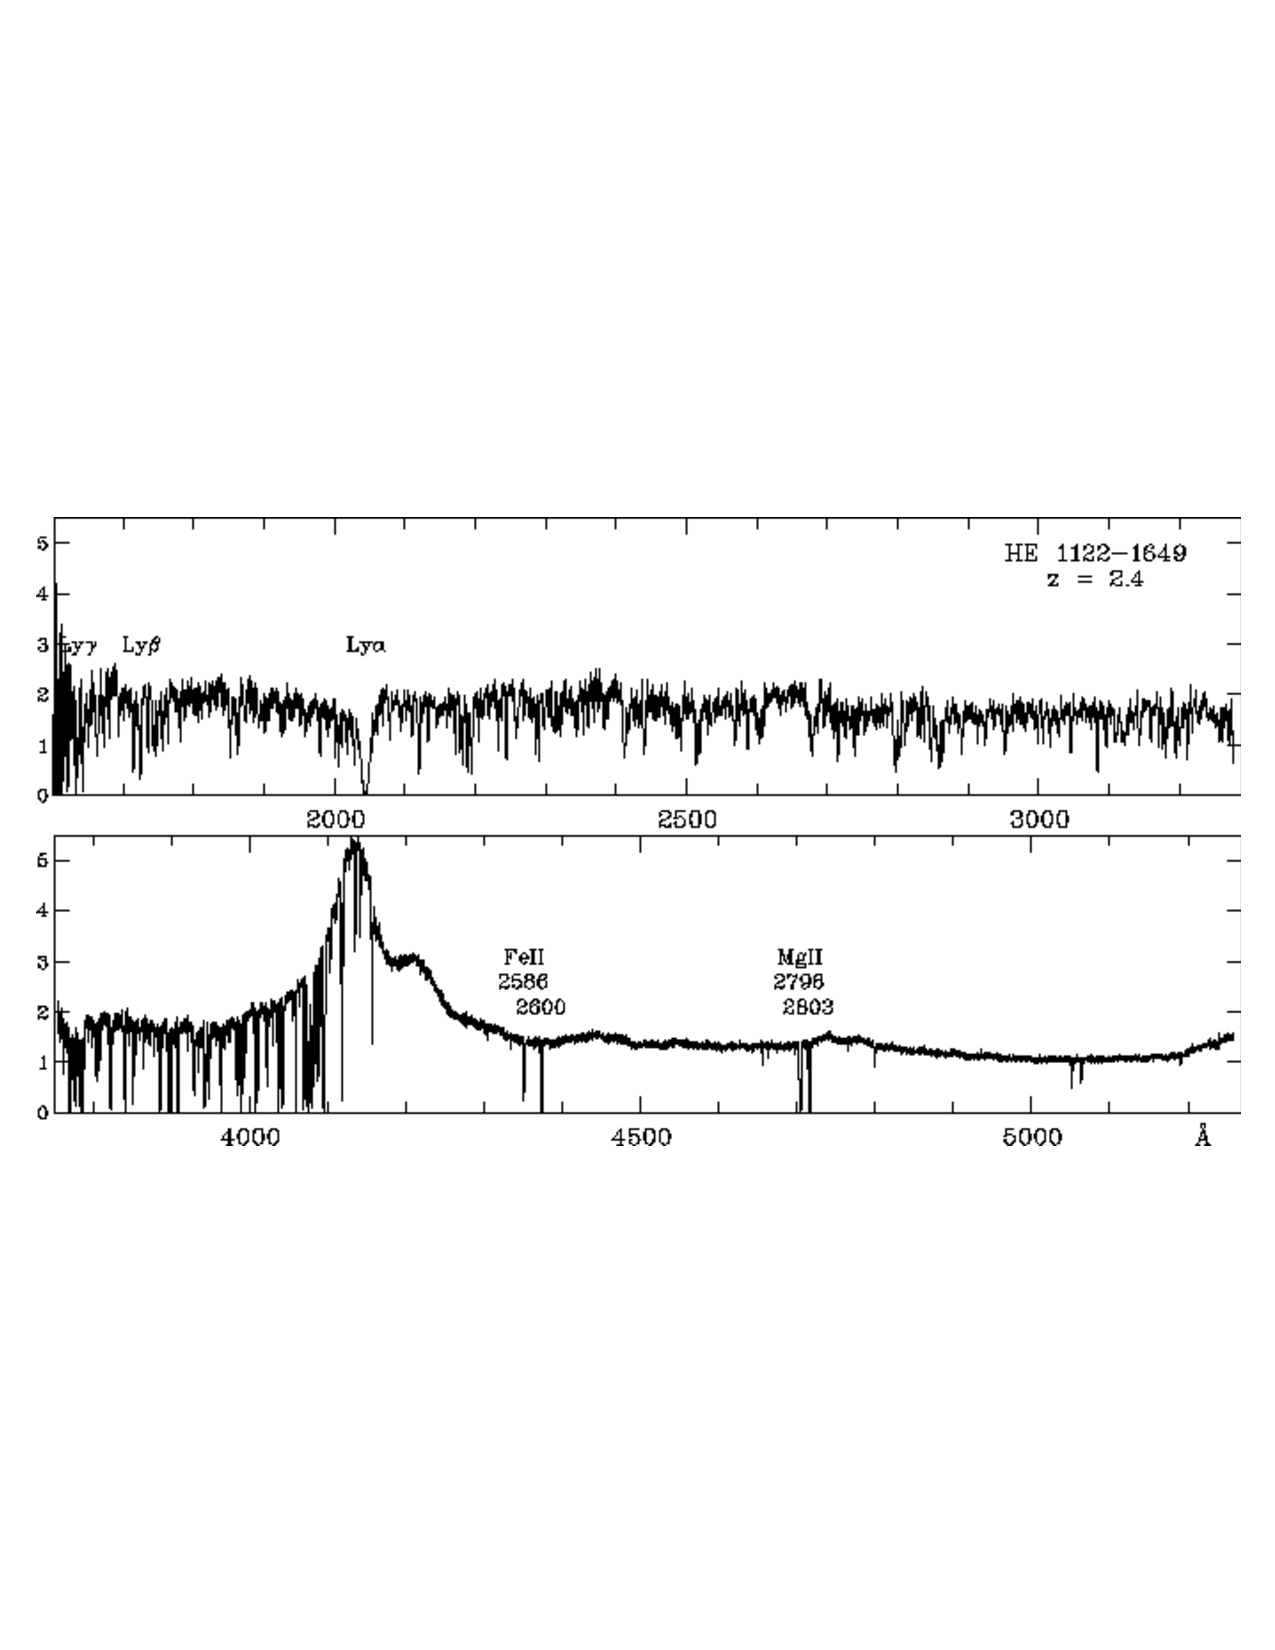
\includegraphics[scale = 0.7, angle=0.0]{ex2_spectrum.pdf}
                  \caption[Fake Caption?]{An exmaple spectrum of a different QSO UV spectrum with a different redshift. The Lyman Alpha and Magnesium II lines are labeled, which should help you find these lines in AO 0235+164's spectrum \footnotemark.}
		\end{center}
		\end{figure}
		\end{center}
         \footnotetext{\it{Absorption line spectra of the UV bright z=2.4 QSO HE 1122-1649}\\
         S. Köhler, A. de la Varga and D. Reimers\\
         Hamburger Sternwarte, Gojenbergsweg 112, 21029 Hamburg, Germany}

	\item What is the Mg~{\sc ii} column density associated with the DLA? Use equation 4.26 as well as the \texttt{splot} task in pyraf. Are the Mg~{\sc ii} lines likely 
		saturated based off what a saturated line looks like in Figure 4.1? What redshift do you derive from the Mg~{\sc ii} doublet? Is it significantly different from
		the redshift derived from H~{\sc i}? Which would you trust more, and why?
	%\item Can you detect Mg~{\sc i} lines? What column density do you derive for Mg~{\sc i}? How accurate do you
	%	think it would be to assume that all of the magnesium in the system is singly ionized?
	\item Zn~{\sc ii} and Cr~{\sc ii} are often used to derive metallicities and dust abundances for DLAs. Can
		you detect lines belonging to either? Hint: Zn~{\sc ii} has rest wavelengths at 2026\AA and 2062\AA(blended) and Cr~{\sc ii} has rest wavelengths at 2056\AA and 2066\AA. Calculate where the observed lines should fall using the redshift in question 1 or 2 of this exercise.
	%\item What other metal lines can you detect with a high degree of confidence? How metal-rich is this DLA based
	%	on these atoms?
         \item Are there any other metal lines you can detect with a high degree of confidence? By calculating the rest wavelengths and using the NIST spectral database or somewhere you can find element emission rest wavelengths and relative intensities, see what these lines likely correspond to. Remember that any airglow lines aren't intrensic to the target and therefore won't be redshifted. How metal-rich would you say this DLA is based on these atoms?
\end{enumerate}